% !TEX TS-program = xelatex
% !TEX encoding = UTF-8 Unicode

% GSET Summer 2021 - Tennessee Technological University
% Tristan Hill - June 16, 2021
% Challenge 6 - Rocket Stability

\documentclass[12pt]{article}

% Custom Preamble
\usepackage{/home/thill/Documents/lectures/cpp_workshop/modules/cpp_tutorial} 

% Title and Misc
\newcommand{\MNUM}{6} %Module Number
\newcommand{\MNAME}{Introduction to C++} %Module Name
\newcommand{\TNAME}{Rocket Stability} %Tutorial Name
\pagestyle{myheadings}
\markright{{\large GSET - Programming with Mr. Hill}}

\begin{document}

\thispagestyle{plain}

\begin{center}
   {\bf \large GSET - Programming with Mr. Hill - Summer 2021} \vspace{5mm}\\
   {\bf \Large \MNAME \hspc -  Challenge\hspc\MNUM\hspc - \TNAME}\vspace{3mm}\\
   
\end{center}

 %\hspace*{3cm}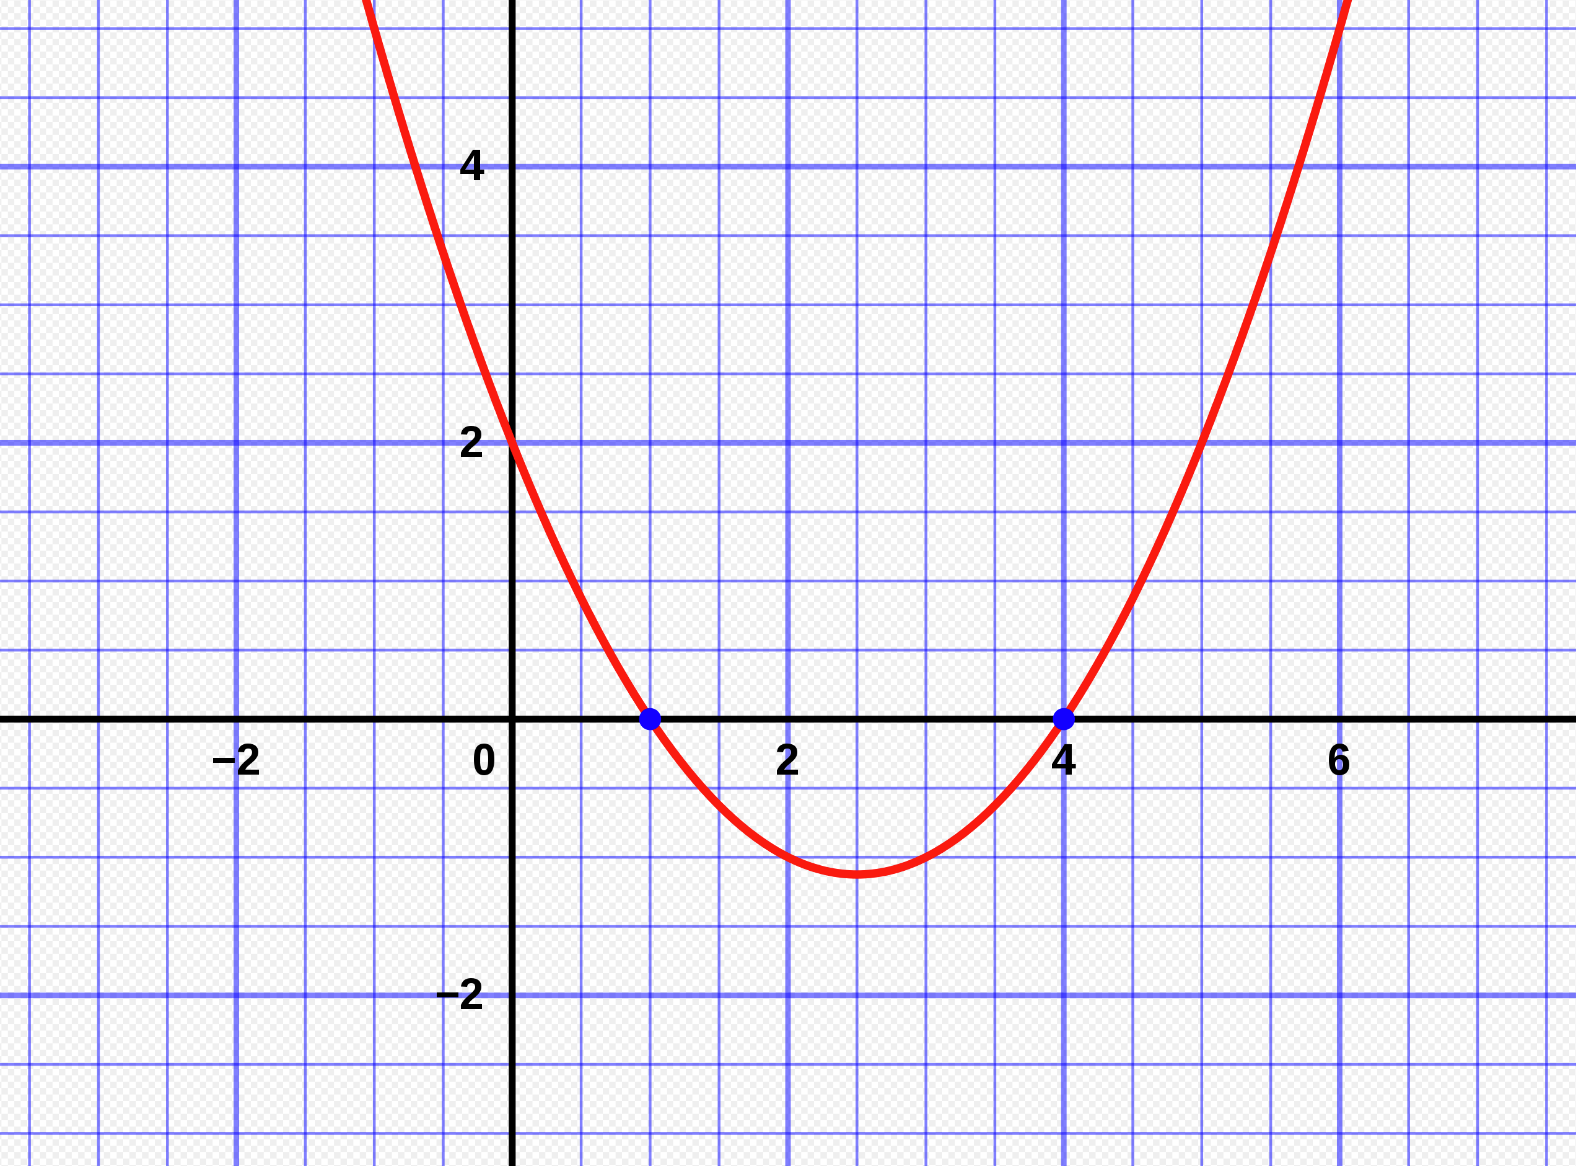
\includegraphics[scale=.15]{quad_equ.png} 

\begin{description}[labelindent=1cm]
	
	\item[\textbf{\underline{Overview:}}] \hfill \vspace{3mm}\\
	We are going to write a C++ program to perform the stability analysis required for the design of a model rocket. This is one way you can help the mission!
	
	\item[\textbf{\underline{System Requirements:}}] \hfill \vspace{0mm}

\begin{itemize}
	\item {\bf Computer}: A computer is required to complete this tutorial. Any OS should work.
	\item {\bf C++:} You can use the online C++ compiler (\href{https://www.onlinegdb.com/online\_c++\_compiler}{OnlineGDB} ) or a C++ compiler of your choice.
\end{itemize}

	\item[\textbf{\underline{Problem Statement:}}] \hfill \vspace{0mm}
	
	\begin{itemize}

		\item Given: The physical properties of the rocket including the dimensions and mass of the individual components 
		
		\item Find: The center of gravity and center or pressure of the proposed design. Also if the rocket is stable, unstable, or quasi-stable.  
		 
	\end{itemize}

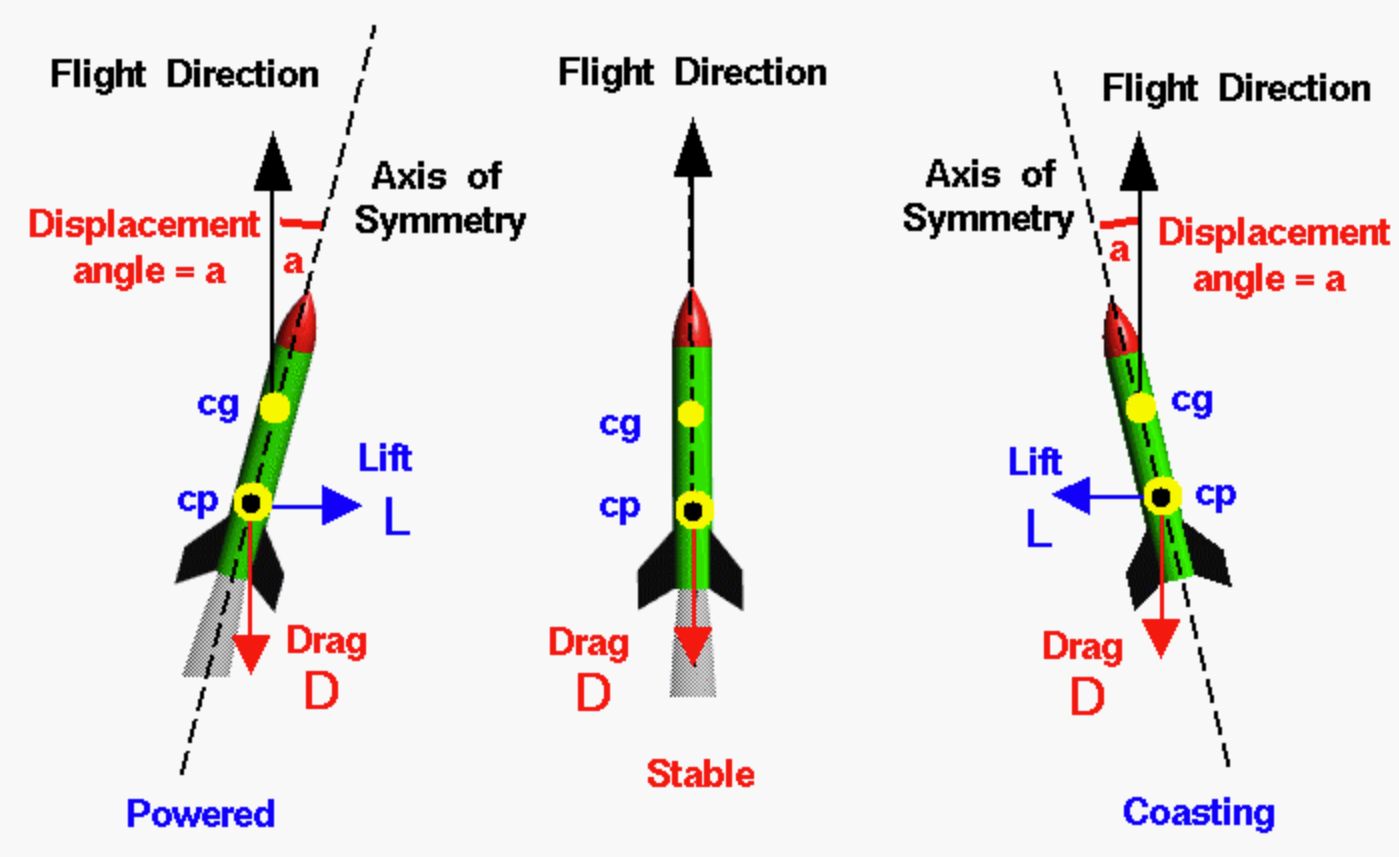
\includegraphics[scale=.3]{rocket_stability.png}


\newpage
\item[\textbf{\underline{Program Minimum Requirements:}}] \hfill \vspace{0mm}

The program should accomplish the following tasks. 


\begin{itemize}

	\item The inputs (rocket parameters) should be stored in your program.

	\item Your program should calculate the center of gravity using the method provided.
	
	\item Your program should calculate the center of pressure using the method provided.
	
	\item Your program should determine whether the input design is stable using the criterion provided.

\end{itemize}	 
	Optional Advanced Features:
\begin{itemize}
	\item The possible range for each input should be stored as an array in your program.
		
	\item there are so many things you could do!
    
\end{itemize}	


%\item[\textbf{\underline{Example Code:}}] \hfill \vspace{0mm}
%\begin{enumerate}
%    \item This is the C style way to output text.
%	%\begin{minted}{cpp}
%	\begin{lstlisting}
%
%// Arrays of Characters - GSET - Summer 2021 
%	
%#include <iostream>
%
%using namespace std;
%
%int main()
%{
%
%	char myname[]={"Tristan"};
%	
%	char c = 'T';
%	
%	cout<<"Hello World\n";
%	
%	cout<<myname<<endl; 
%	
%	cout<<myname[1]<<endl;
%	
%	cout<<(int)c<<"\a" <<endl; 
%	
%	return 0;
%}
%
%
%	\end{lstlisting}
%	%\end{minted}
%		
%\end{enumerate}

	\item[\textbf{\underline{Part 3 - Testing:}}] \hfill \vspace{0mm}
	\begin{enumerate}
	
		\item Develop a  C++ program to the solve the problem described. \\\\
		
		\item Determine a reasonable range for each of the possible inputs. We will discuss this part as a class. \\
		
		\item Use the program you have developed to choose an optimal rocket design. Record the values you chose and document the process you used to determine these values.  \\\\
		
	
		\item Save your code with the download button or use copy and paste. You can view and edit the code in any text editor. Also, save a copy of the program output for your tutorial summary. \\\\

	\end{enumerate}

\newpage
\item[\textbf{\underline{Solution Code:}}] \hfill \vspace{0mm}
%
%\begin{lstlisting}
%
%\end{lstlisting}
%
%\item[\textbf{\underline{Tutorial Complete:}}] \hfill \vspace{3mm}\\ 
%	Congratulations, after completing {\it Tutorial 2 - Quadratic Equation}, you have begun learning to program in C++! You are now ready to start learning about more complex data structures and program flow. \\
%

\newpage
\item[\textbf{\underline{Challenge Summary:}}] \hfill \vspace{3mm}\\ 
Write a brief summary of what you accomplished and what you struggled with the most. 

Include the following items in the summary:
\begin{itemize}

\item a copy of the output of your program
\item a description of what the program does and how to use it

\end{itemize}


%\item[\textbf{\underline{Submission on Teams:}}] \hfill \vspace{3mm}\\ 
%Use the appropriate shared folder on Teams to submit your program and summary. Submit the fol1owing items with your TNTech username in the filenames as shown below. \vspace{0mm}\\
%
%\underline{Files for Tutorial 1 (TNTech Username : twhill21)}
%
%\begin{itemize}
%
%\item Tutorial Summary: \textbf{ twhill21\_summary2.txt}
%
%\item C++ Source Code: \textbf{ twhill21\_tutorial2.cpp}
%
%\end{itemize}


\end{description}
\end{document}

